\documentclass{article}
\usepackage{enumitem}
\usepackage[utf8]{inputenc}
\usepackage{amsmath}
\usepackage{graphicx}

\title{Arsitektur Harvard, Arsitektur von Neumann, ISA, dan Mikro Arsitektur}
\author{}
\date{}

\begin{document}

\maketitle



\section{Arsitektur von Neumann}
John von Neumann pertama kali menawarkan arsitektur von Neumann pada tahun 1945, yang menjadi dasar hampir semua komputer modern. Arsitektur ini terutama memanfaatkan memori yang sama untuk menyimpan data dan instruksi program. Metode ini memungkinkan komputer untuk menjalankan program yang lebih kompleks dan dapat disesuaikan.
\begin{figure}
    \centering
    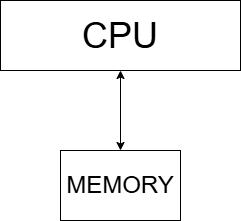
\includegraphics[width=0.5\linewidth]{assets/Van neuman.png}
    \caption{Van Neumann}
    \label{fig:enter-label}
\end{figure}
\subsection{Keuntungan dan Kelemahan}

\begin{enumerate}[label=\arabic*.]
  \item \textbf{Kelebihan:}
  \begin{itemize}
    \item \textbf{Kesederhanaan Desain:}
    \begin{itemize}
      \item Satu Memori untuk Data dan Instruksi: Menggunakan satu ruang memori untuk menyimpan data dan instruksi, menyederhanakan desain sistem memori.
      \item Desain yang Sederhana: Satu set jalur data dan alamat membuat desain perangkat keras menjadi lebih sederhana dan lebih murah.
    \end{itemize}
    
    \item \textbf{Fleksibilitas:}
    \begin{itemize}
      \item Pemrograman yang Fleksibel: Instruksi dan data dapat disimpan dalam memori yang sama, memungkinkan program untuk diubah selama runtime.
      \item Kemudahan Pengembangan \textit{Software}: Perubahan pada kode atau data tidak memerlukan perubahan pada perangkat keras.
    \end{itemize}
    
    \item \textbf{Penggunaan Memori yang Efisien:}
    \begin{itemize}
      \item Penggunaan Memori yang lebih mudah: Memori dapat dialokasikan untuk instruksi atau data sesuai kebutuhan, tanpa harus memisahkan ruang secara fisik.
    \end{itemize}
  \end{itemize}
  
  \item \textbf{Kekurangan:}
  \begin{itemize}
    \item \textbf{Bottleneck Memori (Von Neumann Bottleneck):}
    \begin{itemize}
      \item Kecepatan Transfer yang Terbatas: Satu jalur untuk mengakses memori instruksi dan data bisa menjadi hambatan ketika prosesor mencoba untuk melakukan banyak operasi secara bersamaan, memperlambat kinerja sistem.
    \end{itemize}
    
    \item \textbf{Performa yang Kurang Optimal:}
    \begin{itemize}
      \item Akses Memori yang Bersama: Proses pengambilan instruksi dan akses data harus dilakukan secara bergantian, yang dapat mengurangi kecepatan eksekusi jika kedua jenis operasi terjadi secara bersamaan.
    \end{itemize}
    
    \item \textbf{Keamanan dan Stabilitas:}
    \begin{itemize}
      \item Risiko Kesalahan Pengkodean: Karena data dan instruksi disimpan bersama, kesalahan dalam penanganan data atau instruksi dapat menyebabkan masalah seperti corrupt data atau instruksi.
    \end{itemize}
  \end{itemize}
\end{enumerate}

\section{Arsitektur Harvard}

Arsitektur Harvard menggunakan dua ruang memori yang berbeda untuk menyimpan instruksi dan data, berbeda dengan arsitektur von Neumann. Ini memungkinkan pengambilan instruksi dan data secara bersamaan, yang dapat meningkatkan kinerja dan efisiensi sistem.
\begin{figure}
    \centering
    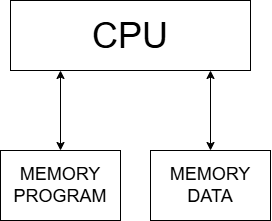
\includegraphics[width=0.5\linewidth]{assets/Harvard.png}
    \caption{Harvard}
    \label{fig:enter-label}
\end{figure}
\subsection{Kelebihan}

\begin{enumerate}[label=\arabic*.]
  \item \textbf{Performa Lebih Baik:}
  \begin{itemize}
    \item Akses Memori Paralel: Memiliki jalur terpisah untuk data dan instruksi memungkinkan akses simultan ke memori instruksi dan data, meningkatkan kecepatan eksekusi dan mengurangi bottleneck memori.
    \item Eksekusi Instruksi yang Lebih Cepat: Dengan akses yang terpisah, \textit{prosesor} dapat mengambil instruksi dan data secara bersamaan, mempercepat kinerja sistem.
  \end{itemize}
  
  \item \textbf{Optimasi Memori:}
  \begin{itemize}
    \item Pengaturan Memori yang Terpisah: Memori instruksi dan data yang terpisah memungkinkan optimasi yang lebih baik untuk masing-masing, seperti menggunakan cache yang berbeda untuk instruksi dan data.
  \end{itemize}
  
  \item \textbf{Keamanan dan Stabilitas:}
  \begin{itemize}
    \item Isolasi Data dan Instruksi: Dengan memisahkan data dan instruksi, risiko kesalahan pengkodean yang dapat menyebabkan data bisa rusak atau instruksi berkurang.
  \end{itemize}
\end{enumerate}

\subsection{Kekurangan}

\begin{enumerate}[label=\arabic*.]
  \item \textbf{Kompleksitas Desain:}
  \begin{itemize}
    \item Desain yang Lebih sulit: memakai dua jalur memori terpisah dan pengaturan memori yang lebih kompleks, yang dapat meningkatkan biaya dan kompleksitas desain perangkat keras.
    \item Penggunaan Memori yang Tidak Fleksibel: Memori untuk instruksi dan data harus dialokasikan secara terpisah, yang bisa menyebabkan pemborosan jika salah satu jenis memori tidak digunakan sepenuhnya.
  \end{itemize}
  
  \item \textbf{Kesulitan dalam Pengembangan:}
  \begin{itemize}
    \item Pengembangan Perangkat Lunak yang Lebih Kompleks: Memerlukan pemisahan antara data dan instruksi dalam pemrograman, yang dapat menambah kompleksitas pengembangan perangkat lunak.
  \end{itemize}
  
  \item \textbf{Keterbatasan dalam Adaptasi:}
  \begin{itemize}
    \item Kurang Fleksibel: Penambahan atau perubahan pada memori instruksi atau data mungkin memerlukan perubahan perangkat keras, mengurangi fleksibilitas dalam pembaruan atau peningkatan sistem.
  \end{itemize}
\end{enumerate}

\section{Instruction Set Architecture (ISA)}
(ISA)Instruction Set Architecture atau Arsitektur Set Instruksi adalah bagian dari arsitektur komputer yang menentukan cara kerja perangkat keras dan perangkat lunak dalam menjalankan instruksi program. ISA berperan sebagai jembatan antara perangkat lunak (software) dan perangkat keras (hardware) dalam sistem komputer.
\begin{figure}
    \centering
    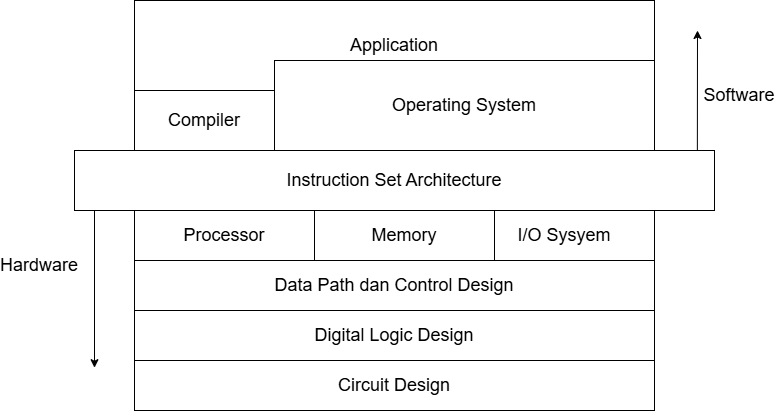
\includegraphics[width=1\linewidth]{assets/ISA.drawio.png}
    \caption{Arsitektur Set Instruksi}
    \label{fig:enter-label}
\end{figure}
\subsection{Komponen Utama ISA}

\begin{itemize}
  \item Set Instruksi: Kumpulan perintah yang dapat dijalankan oleh \textit{prosesor}.
  \item Mode Pengalamatan: Cara dalam menentukan lokasi data yang diperlukan oleh instruksi.
  \item Format Instruksi: Tata letak atau struktur instruksi di dalam memori.
\end{itemize}

\subsection{Jenis-Jenis ISA}

\begin{enumerate}[label=\arabic*.]
  \item \textbf{CISC (\textit{Complex Instruction Set Computing atau Komputasi Set Instruksi Kompleks}):} Set instruksi yang lebih kompleks dengan tujuan untuk mengurangi jumlah instruksi yang perlu dieksekusi oleh \textit{prosesor}.
  \item \textbf{RISC (\textit{Reduced Instruction Set Computing atau Pengurangan Komputasi Set Instruksi}):} Set instruksi yang lebih sederhana, tetapi dapat dieksekusi dengan cepat oleh \textit{prosesor}.
\end{enumerate}

ISA itu penting karena menentukan performa \textit{prosesor} serta kemampuannya dalam menjalankan berbagai aplikasi perangkat lunak.

\section{Mikro Arsitektur}

Mikro arsitektur adalah desain internal \textit{prosesor} yang mencakup semua bagian, seperti unit kontrol, unit aritmatika dan logika (ALU), dan cache memori. Ini melibatkan implementasi fisik dari ISA. Mikro arsitektur bertujuan untuk membuat \textit{prosesor} menangani dan menjalankan instruksi seefektif mungkin.

\subsection{Komponen Utama Mikro Arsitektur}

\begin{itemize}
  \item \textbf{\textit{Pipelining}:} Teknik untuk meningkatkan efisiensi \textit{prosesor} dengan mengeksekusi beberapa instruksi sekaligus pada berbagai tahap pemrosesan.

  \item \textbf{\textit{Branch Prediction}:} Teknologi yang memungkinkan \textit{prosesor} untuk memprediksi cabang dari instruksi kondisional sehingga dapat mengurangi penundaan dalam eksekusi.
\end{itemize}

Mikro arsitektur berfungsi sebagai penghubung antara ISA dan desain perangkat keras, yang berarti bahwa implementasi fisik dari sebuah \textit{prosesor} dapat bervariasi meskipun memiliki ISA yang sama.

\section{Kesimpulan}

Arsitektur sebuah sistem komputer sangat penting untuk kinerja, efisiensi, dan fleksibilitasnya. Setiap metode arsitektur von Neumann dan Harvard untuk menangani data dan instruksi memiliki kelebihan dan kekurangan. Sementara Arsitektur Set Instruksi berfungsi sebagai jembatan antara perangkat lunak dan perangkat keras, mikro arsitektur berkonsentrasi pada desain fisik \textit{prosesor} untuk melaksanakan ISA. Memahami perbedaan dan manfaat masing-masing arsitektur ini sangat penting untuk mengembangkan dan mengoptimalkan sistem komputer.

\section{Referensi}

\begin{enumerate}
  \item Hennessy, J. L., \& Patterson, D. A. (2011). \textit{Computer Architecture: A Quantitative Approach}. Morgan Kaufmann.
  \item Stallings, W. (2015). \textit{Computer Organization and Architecture: Designing for Performance}. Pearson.
  \item UNIKOM.M Zusane Oematan (2010).  \textit{Ringkasan Set Instruksi Dan Mode pengalamatan (Addressing Mode }. 
\end{enumerate}

\end{document}
